\documentclass[a4j,dvipdfmx]{jsarticle}
\usepackage{amsmath,amssymb}
\usepackage{siunitx}
\usepackage[dvips]{graphicx}
\usepackage{listings}
\begin{document}
\section*{数値積分法}
\subsection*{定積分の近似値}
定積分の値は、不定積分がわかれば簡単に計算できる\footnote{微積分学の基本定理より$F(b)-F(a)$}。しかし、不定積分が求められない場合も多い。
たとえば、
\begin{equation*}
    \int e^{-x^2}dx
\end{equation*}
を求めようと思っても、初等関数では表せないのだ(初等関数以外では表せる場合もあるが)。

ここでは、近似公式や計算機を使って定積分の近似値を求める方法(\textgt{数値積分法})を簡単に紹介する。詳しく知りたい場合は専門書等を見てくだせえ。

定積分$\int_a^b f(x)dx$の近似値は、積和$S_n=\sum_{k=1}^n f(\zeta_k)\Delta_k$によって計算できる。n個
の'帯'に分けるとき、その帯をどのように近似するかによって、種々の公式を得られる。
\subsection{台形公式}
曲線$y=f(x),x=a,x=b$ x軸で囲まれる面積を、幅$h=(b-a)/n$のn個の帯に分割する。i番目の帯の上部は弧$P_{i-1}P_i$
であるが、これを直線で結び、面積を
\begin{equation}
 \frac{1}{2}h{f(a+(i-1)h)+f(a+ih)}   
\end{equation}
で近似する。各々の帯の面積をこのように近似して、\textgt{台形公式}
\begin{align}
    \int_a^b f(x)dx&\fallingdotseq \frac{h}{2}(f(a)+f(a+h))+\frac{h}{2}(f(a+h)+f(a+2h))+\cdots+\frac{h}{2}(f(a+(n-1)h)+f(b))\\
    \label{trapezeopdal rule}
    &\fallingdotseq\frac{h}{2}(f(a)+2f(a+h)+2f(a+2h)+\cdots+2f(a+(n-1)h)+f(b))
\end{align}
を得る。
\begin{figure}[h]
    \centering
    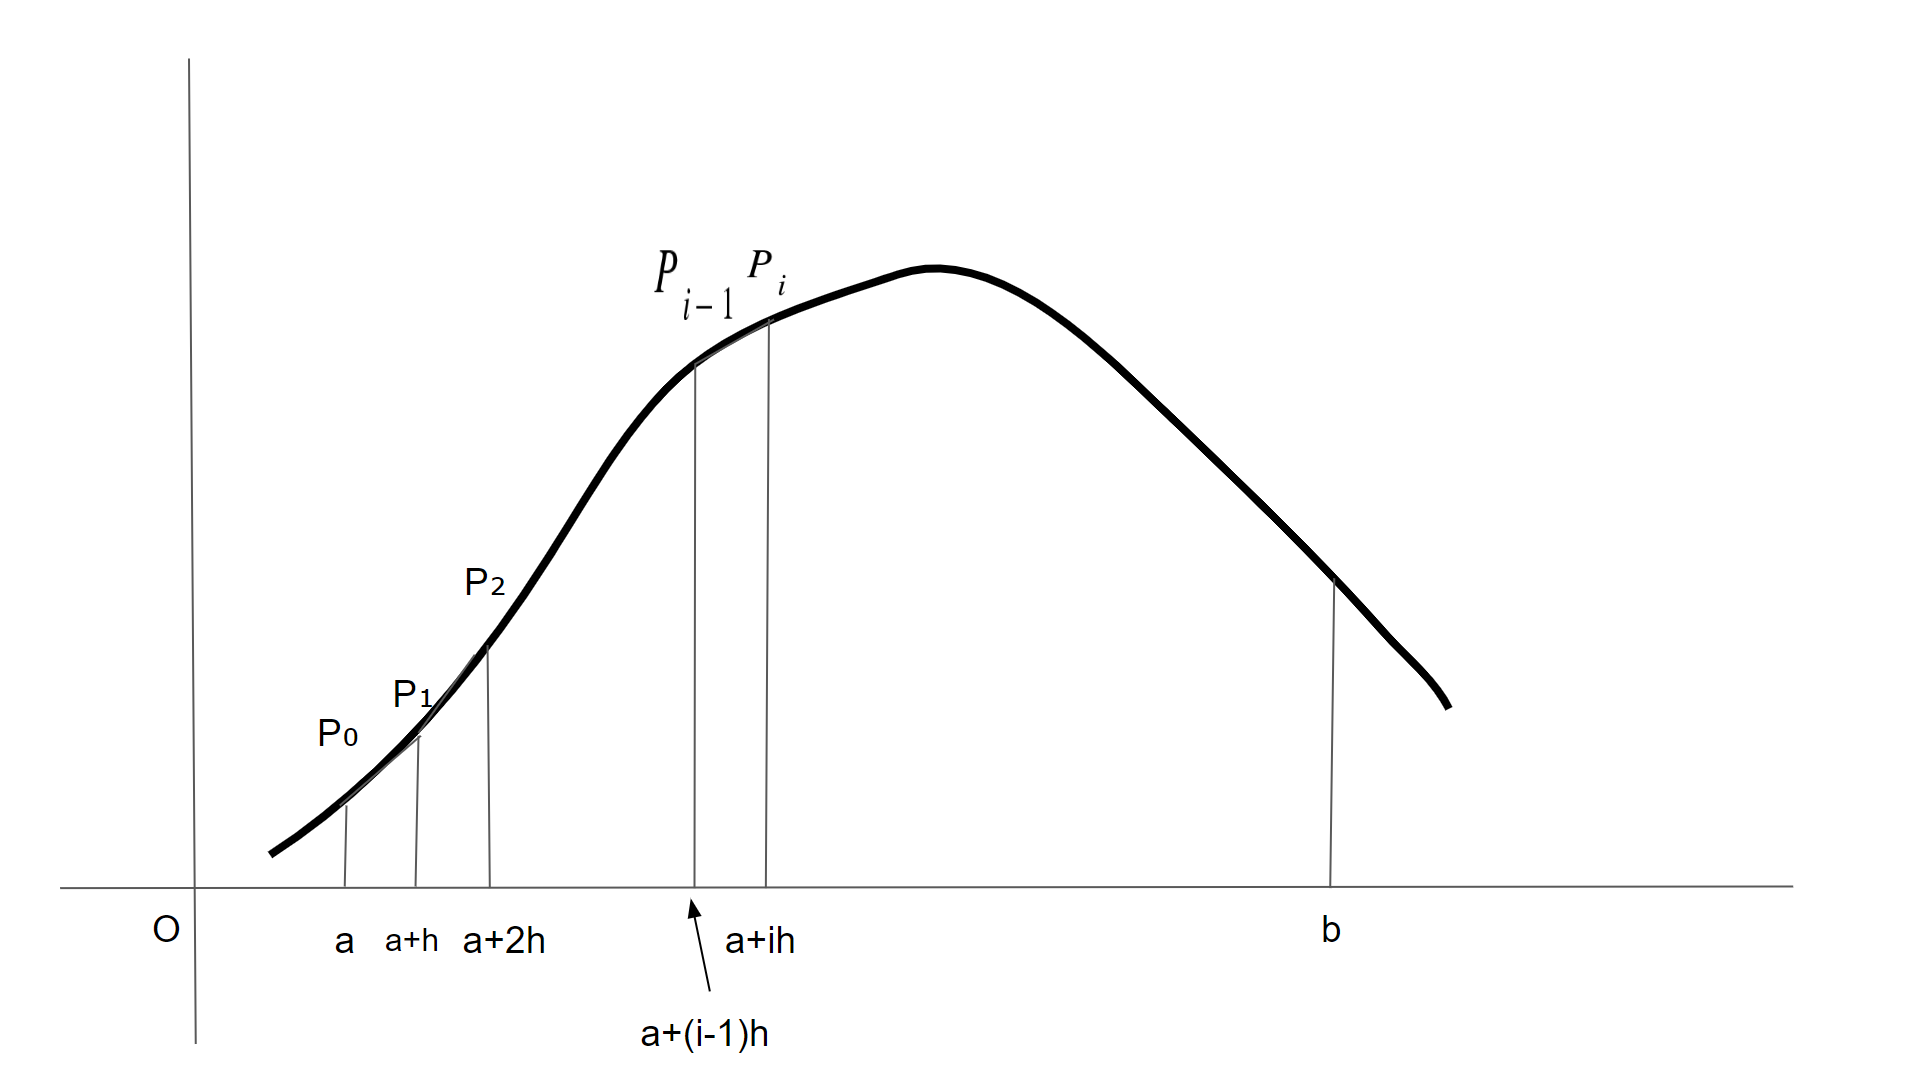
\includegraphics[width=10cm,scale=5]{img/trapezoidal_rule.png}
    \caption{台形公式}
\end{figure}
\newpage
\subsection{シンプソンの公式}
今度は、面積を幅$h=(b-a)/2m$の$n=2m$個の帯に分割する。その帯を2個ずつまとめて、弧$P_0P_1P_2,P_2P_3P_4,\cdots,P_{2m-2}P_{2m-1}P_{2m}$を持つ$m$個の帯を作る\footnote{残念ながら図はない。作るのが面倒だった。興味があったらインターネットで調べて。}。
$i$番目の帯の上部は弧$P_{2i-1}P_{2i-1}P_{2i}$であるが、これを通る放物線$y=Ax^2+Bx+C$で近似すると、面積は
\begin{equation}
    \frac{h}{3}(f(a+2(i-2)h)+4f(a+(2i-1)h)+f(a+2ih))
\end{equation}
となる(下の例題)。$m$個の帯の面積をこのように近似して、\textgt{シンプソンの公式}
\begin{align}
    \label{simpson}
    \int_a^b f(x)dx\fallingdotseq &\frac{h}{3}(f(a)+4f(a+h)+2f(a+2h)+4f(a+3h)+2f(a+4h)\notag\\
    &+\cdots+2f(a+(2m-2)h)+4f(a+(2m-1)h)+f(b))
\end{align}
を得る。\\\\
\subsubsection*{例題1}
3点$P_0(a,y_0),P_1(\frac{a+b}{2},y_1),P_2(b,y_2)$を通る放物線$y=Ax^2+Bx+C$に対して、
\begin{equation*}
    \int_a^b ydx=\frac{b-a}{6}(y_0+4y_1+y_2)
\end{equation*}
を示せ。\\\\
\subsubsection*{解答}
定積分の値は
\begin{equation*}
    \int_a^b ydx=\int_a^b(Ax^2+Bx+C)dx=\frac{b-a}{3}(A(a^2+ab+b^2)+\frac{3}{2}B(a+b)+3C)
\end{equation*}
$y=Ax^2+Bx+C$は3点$P_0,P_1,P_2$を通るから、
\begin{align*}
    y_0&=Aa^2+Ba+C\\
    y_1&=A(\frac{a+b}{2})^2+B\frac{a+b}{2}+C\\
    y_2&=Ab^2+Bb+C
\end{align*}
よって、
\begin{equation*}
    y_0+4y_1+y_2=2(A(a^2+ab+b^2)+\frac{3}{2}B(a+b)+3C)
\end{equation*}
だから、
\begin{equation*}
    \int_a^b ydx=\frac{b-a}{6}(y_0+4y_1+y_2)
\end{equation*}
\newpage
電卓を用いて、次の例題を解いてみよう。
\subsubsection*{例題2}
定積分$\int_0^1e^{-x^2}dx$を$n=10$の、(a)台形公式、(b)シンプソンの公式、を用いて計算せよ。
\subsubsection*{解}
$h=0.1$である。あらかじめ、$f(x)=e^{-x^2}$の値を計算しておく。(表でまとめると便利\footnote{余談だが、表1を描画するのにすごく苦労した})\\
\begin{table*}[h]
    \caption{$e^{-x^2}$の値}
    \begin{tabular}{|c||c|c|c|c|c|} \hline
        x    & 0    & 0.1        & 0.2        & 0.3        & 0.4        \\ \hline
        f(x) & 1    &0.990049834 &0.960789439 &0.913931185 &0.852143789 \\ \hline
    \end{tabular}
    \\\\
    \begin{tabular}{|c||c|c|c|c|c|c|} \hline
        x    & 0.5        & 0.6        & 0.7        & 0.8        & 0.9        & 1  \\ \hline
        f(x) &0.778800783 &0.697676326 &0.612626394 &0.527292424 &0.444858066 &0.367879441 \\ \hline
    \end{tabular} 
\end{table*}
%  & 0.5        & 0.6        & 0.7        & 0.8        & 0.9        & 1
% &0.778800783 &0.697676326 &0.612626394 &0.527292424 &0.444858066 &0.367879441
\\
(a)台形公式(\ref{trapezeopdal rule})より
\begin{align*}
    \int_0^1e^{-x^2}dx&=\frac{0.1}{2}(f(0)+2f(0.1)+2f(0.2)+2f(0.3)+2f(0.4)+2f(0.5)+2f(0.6)+2f(0.7)+2f(0.8)+2f(0.9)+f(1))\\
                      &=0.746211
\end{align*}
(b)シンプソンの公式(\ref{simpson})より
\begin{align*}
    \int_0^1e^{-x^2}dx&=\frac{0.1}{3}(f(0)+4f(0.1)+2f(0.2)+4f(0.3)+2f(0.4)+4f(0.5)+2f(0.6)+4f(0.7)+2f(0.8)+4f(0.9)+f(1))\\
                      &=0.746825
\end{align*}
なお、正確な値を小数第六桁まで書くと$0.746825$である。\\
\subsubsection*{問題}
以下それぞれ(a)台形公式と(b)シンプソンの公式を用いて計算し、正しい積分値と比べよ。
\begin{align*}
    1.&\int_2^6\frac{dx}{x} &\cdots((a)n=4,(b)n=4)& \\
    2.&\int_0^{\frac{1}{2}}\frac{dx}{1+x^2} &\cdots((a)n=5,(b)n=4)&
\end{align*}
\newpage
\subsection*{最後に}
今回は数値積分法について軽く触れた。不定積分が求められなくても、定積分の値なら求められることがあることがわかっただろう。\\

次回は関数の展開とオイラーの公式について触れる。先にネタバレをしてしまうと、関数の展開はその名前の通り関数を有理関数の和に展開することである。例えば
$\sin x$を展開すると
\begin{equation*}
    \sin x=x-\frac{x^3}{3!}+\frac{x^5}{5!}+\cdots+\frac{(-1)^{n-1}x^{2n-1}}{(2n-1)!}+R_{2n+1},R_{2n+1}=(-1)^n\frac{x^{2n-1}}{(2n-1)!}\cos\theta x\cdots(0<\theta<1)
\end{equation*}
となる。なぜこのようになるのかは次回の楽しみにしておいてほしい。\\
オイラーの公式はこの関数の展開を利用して導くもので、式は
\begin{equation*}
    e^{ix}=\cos x+i\sin x
\end{equation*}
と、三角関数の和が指数関数になってしまうのである。アメリカの物理学者リチャード・ファインマンはこの式を\textgt{人類の至宝}といったらしい。
ちなみに$x=\pi$とすると直ちに
\begin{equation*}
    e^{i\pi}+1=0
\end{equation*}
が成り立つ\footnote{$\cos \pi=-1,\sin \pi=0$より}。またこの公式を用いれば、有名なド・モアブルの公式も簡単に示せてしまうのだが、それは次の機会に取っておこう。

話がそれてしまったが、残すところ積分も最後である(まぁ二年生になったら多変数の微分積分をやるのだが)。気を引き締めていきたい。
\footnote{メモ:(制作時間 約3時間)正月早々なにやってんだ}
\newpage
\subsection*{おまけ}
数値積分のソースコード。問題(1)の計算をJava(OpenJDK17)で実装した。

\lstset{
    frame=single,
    numbers=left,
    language=java,
}

\begin{lstlisting}[caption=Main.java,]
    package javas.lab;

    import javas.maths.*;
    
    public class Main {
        public static void main(String[] args) {
            System.out.println(integral.simpson_rule(new Function() {
                @Override
                public double func(double x) {
                    return 1/x;
                }   
                @Override
                public boolean isEvenFunction() {
                    return false;
                }
                @Override
                public boolean isOddFunction() {
                    return true;
                }
            }, 2, 6, 4));
        }
    
    }
\end{lstlisting}
\begin{lstlisting}[caption=Function.java]
    package javas.maths;

public interface Function {
    public double func(double x);
    // 偶関数かどうか
    public boolean isEvenFunction();
    // 奇関数かどうか
    public boolean isOddFunction();
}
\end{lstlisting}
\newpage
\begin{lstlisting}[caption=integral.java]
    package javas.maths;

public class integral {
    /**
     * 
     * @param fx    :被積分関数
     * @param begin :積分下限
     * @param end   :積分上限
     * @param n :帯の数 多ければ多いほどよい近似値が得られる
     * @return 台形公式による定積分の近似値
     */
    public static double trapezoidal_rule(Function fx,
                                            double begin,double end,int n){
        if(begin==end)return 0;
        if(fx.isOddFunction()&&begin==-end)return 0;

        double sum=0;
        double width=(end-begin)/n;

        for(double i=begin;i<=end;i+=width){
            sum+=fx.func(i);
            if(!(i==begin||i==end))sum+=fx.func(i);
        }
        sum*=width/2;
        return sum;
    }
    /**
     * 
     * @param fx    :被積分関数
     * @param begin :積分下限
     * @param end   :積分上限
     * @param n :帯の数 多ければ多いほどよい近似値が得られる
     * @return シンプソンの公式による定積分の近似値
     */
    public static double simpson_rule(Function fx,
                                        double begin,double end,int n) {
        if(begin==end)return 0;
        if(fx.isOddFunction()&&begin==-end)return 0;

        double sum=0;
        double width=(end-begin)/n;

        for (int i = 0; i < n+1; i++) {
            double temp;
            temp=fx.func(begin+i*width);
            if(!(i==0||i==n))temp*= i%2==0?2:4;
            sum+=temp;
        }
        sum*=width/3;
        return sum;
    }
}
\end{lstlisting}

シンプソンの公式を使っているが、台形公式でも計算できる。その場合は12行目の「trapezoidal」を「simpson」に変えるだけだ。
\newpage

Mainクラスのmainメゾット内にある匿名クラス宣言しているコードを書き換えれば、別の関数でも計算することができる。

例えば、$e^x$を計算したいとしたら

\begin{lstlisting}
    ...
    public static void main(String[] args) {
        System.out.println(integral.simpson_rule(new Function() {
            @Override
            public double func(double x) {
                return Math.exp(x);
            }   
            @Override
            public boolean isEvenFunction() {
                return false;
            }
            @Override
            public boolean isOddFunction() {
                return false;
            }
        }, 2, 6, 4));
    }
    ...
\end{lstlisting}
とすればよい。このときisEvenFunction()とisOddFunction()を書き換えることを忘れないようにしよう。

正直に言って、Javaは数値計算するための言語ではないが、残念なことに私はJava以外の言語はあまり触れたことがないのだ。\footnote{Pythonを使えば簡単にできるだろうが、PythonのほうがJavaより動作が遅い!}

このソースコードは自由に改変してもらって構わない。もしコードに間違いがあったら指摘してほしい。\footnote{コードが汚いとしても黙っていてほしい(笑)}
ソースコードはsrcフォルダにおいておく。
\end{document}